\subsection{Base radiale (RBF)}
\subsubsection*{Neurone}
Un neurone d'un \rbf n'effectue pas de somme pondérée de ses entrées. Il applique directement sa fonction \[\phi(x) = e^{-\beta||x-\mu||^2}\]
Où $x$ est l'entrée, $\mu$ le prototype, $\beta$ le coefficient qui règle la largeur de la courbe en cloche. $x$ et $\mu$ sont des vecteurs.
\begin{figure}
 \centering
 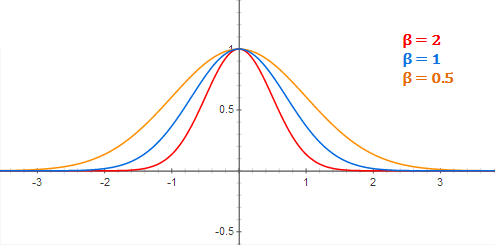
\includegraphics[scale=0.7]{../figures/RBFactivation.png}
 \caption{Activation d'un neurone RBF avec différentes valeurs pour $\beta$}
 \label{rbfactivation}
\end{figure}
La Figure \ref{rbfactivation} représente la sortie d'un neurone \rbf où $\mu$ et $x$ sont de dimension 1 et $\mu = 0$.\\
Pour résumer, un neurone \rbf renvoie une valeur indiquant la simularité entre l'entrée et son prototype.
\subsubsection*{Structure}
\begin{figure}
 \centering
 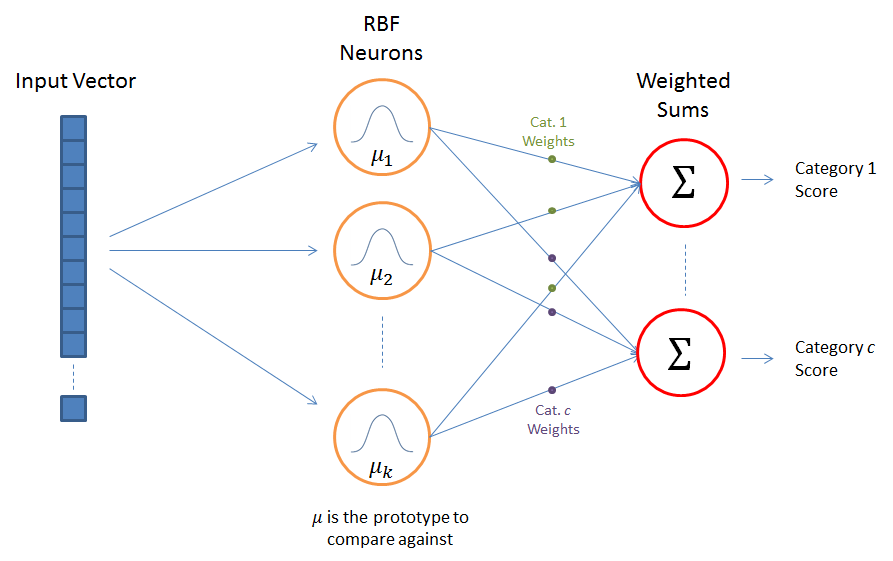
\includegraphics[scale=0.5]{../figures/RBFstruct.png}
 \caption{Structure RBF. \textbf{Source}: McCormick\cite{RBFtuto}}
 \label{structurerbf}
\end{figure}
La structure d'un \rbf est comme celle du \mlp sauf qu'il n'y a qu'une seule couche cachée (Figure \ref{structurerbf}).
\subsubsection*{Applications}
Un \rbf peut aussi servir dans la prédiction de profil.\cite{statistica}